\section{Baseline Results}

\subsection{Main Finding: Primary-Backbone TTA Failure on Real WiFi CSI}

\begin{table}[t]
\centering
\caption{Decision table (primary MLP backbone, $n{=}15$ per method). For each dataset we report source-only accuracy, the best and worst TTA method (mean gain and 95\% bootstrap CI for best; gain only for worst), the negative-adaptation rate of the best method, and the source-domain drop of that method. On the primary MLP, no method's 95\% CI clears zero on any real dataset; \texttt{selective\_physics} is consistently least harmful. Full per-method tables per dataset are in Appendix~\ref{app:per_method_full}.}
\label{tab:decision}
\small
\setlength{\tabcolsep}{4pt}
\resizebox{\textwidth}{!}{%
\begin{tabular}{llcccccc}
\toprule
\textbf{Dataset} & \textbf{Backbone} & \textbf{no\_adapt} & \textbf{Best TTA (gain, 95\% CI)} & \textbf{Worst TTA (gain)} & \textbf{Neg rate} & \textbf{Src drop} \\
\midrule
Widar\_BVP & MLP & 37.3\% & \texttt{selective\_phys} $+$0.3~pp $[-0.3,+0.8]$ & \texttt{sar} $-$7.6~pp & 0.33 & $-$1.5~pp \\
NTU-Fi HAR & MLP & 69.7\% & \texttt{tent-proj} $-$0.6~pp $[-1.3,+0.1]$ & \texttt{entropy} $-$18.9~pp & 0.53 & $-$0.1~pp \\
SignFi-10 & MLP & $\sim$95\% & \texttt{selective\_phys} $-$0.8~pp $[-2.0,+0.0]$ & \texttt{im} $-$12.4~pp & 0.13 & --- \\
\midrule
Synthetic & MLP & --- & \texttt{safe\_physics} $+$8.0~pp & \texttt{entropy} $\approx$0~pp & 0.07 & --- \\
\bottomrule
\end{tabular}%
}
\end{table}

Table~\ref{tab:decision} presents the central primary-backbone finding: \emph{on the primary MLP backbone, no method's 95\% CI clears zero on any of the three real datasets}. Entropy-based methods incur $-$13.8 to $-$15.1~pp mean source-domain degradation on Widar, while \texttt{selective\_physics} keeps source drop to $-$1.5~pp. The cross-dataset rank correlation across the seven methods evaluated on all three datasets has mean Spearman $\rho{\approx}0.70$ (computed by \texttt{scripts/analyze\_tta\_adaptation.py}). Per-method and per-room Widar tables, the leaderboard, step-budget and threshold-sensitivity studies, and the confusion-matrix visualisation (Figure~\ref{fig:confusion}, previously in main) are in Appendices~\ref{app:per_method_full}, \ref{app:per_room}, \ref{app:step_budget}, and \ref{app:threshold_sensitivity}.

\subsection{Cross-Dataset SAR / CoTTA / LAME and the Simplified-vs-Faithful Port}

Recent TTA methods (SAR, CoTTA, LAME) rely on BatchNorm-affine updates or parameter-free output adjustment; porting them to our shared primary-MLP backbone required simplifications. To test whether the simplifications drive the negative results we add (i) the simplified-MLP port on all three datasets and (ii) the faithful BN-only SAR/CoTTA and full TENT on an MLP+BN backbone on Widar\_BVP at $n{=}15$.

\begin{table}[h]
\centering
\caption{Cross-dataset SAR / CoTTA / LAME ($n{=}15$). The faithful MLP+BN block shows that the large $-$7.6\,/\,$-$6.6~pp simplified-MLP numbers on Widar partly reflect the port, not a universal method failure; the faithful numbers shrink to $-$0.15\,/\,$-$0.38~pp and overlap zero, but still do not exceed the BN-only TENT control that also fails. LAME in our shared-backbone port is parameter-free and leaves predictions unchanged. Full table including NegRate in Appendix~\ref{app:coverage}.}
\label{tab:lame_sar_cotta_main}
\small
\setlength{\tabcolsep}{4pt}
\resizebox{\textwidth}{!}{%
\begin{tabular}{llccc}
\toprule
\textbf{Dataset / Port} & \textbf{Method} & \textbf{Gain (pp)} & \textbf{95\% CI (pp)} & \textbf{NegRate} \\
\midrule
\multirow{3}{*}{Widar\_BVP (MLP, simplified)}  & sar   & $-$7.62  & $[-9.86,\,-5.43]$  & 0.93 \\
                                               & cotta & $-$6.58  & $[-9.42,\,-3.78]$  & 0.80 \\
                                               & lame  & $\phantom{+}0.00$ & $[\phantom{-}0.00,\,\phantom{+}0.00]$ & 0.00 \\
\midrule
\multirow{3}{*}{Widar\_BVP (MLP+BN, faithful)} & sar   & $-$0.15 & $[-0.69,\,+0.43]$ & 0.73 \\
                                               & cotta & $-$0.38 & $[-0.84,\,+0.12]$ & 0.73 \\
                                               & tent (faithful, BN-only) & $-$0.01 & $[-0.37,\,+0.35]$ & 0.47 \\
\midrule
NTU-Fi (MLP, simplified)                       & sar   & $-$17.69 & $[-21.43,\,-14.18]$ & 1.00 \\
NTU-Fi (MLP, simplified)                       & cotta & $-$17.67 & $[-20.71,\,-14.46]$ & 1.00 \\
\midrule
SignFi-10 (MLP, simplified)                    & sar   & $-$11.81 & $[-17.90,\,-6.51]$  & 0.73 \\
SignFi-10 (MLP, simplified)                    & cotta & $-$12.38 & $[-18.32,\,-6.92]$  & 0.73 \\
\bottomrule
\end{tabular}%
}
\end{table}

The faithful-port rows answer the main baseline-fairness objection to the decision table: on an MLP+BN Widar backbone, SAR and CoTTA are neither harmful nor helpful (CIs overlap zero); faithful BN-only TENT on the same backbone is essentially zero ($-$0.01\,pp). The SignFi MLP+BN counterexample ($+$21.1\,pp; Table~\ref{tab:signfi_mlpbn}) therefore cannot be attributed to SAR/CoTTA being mis-ported, and the larger negative numbers on the simplified primary MLP port remain a legitimate harm-aware signal for deployers who cannot change the backbone.

\subsection{Per-Class Overconfidence Evidence}

Table~\ref{tab:overconfidence_main} anchors the overconfidence claim in the intro and Mechanism~1: the source model assigns $\geq 70$\,\% mean confidence to every Widar class while per-class accuracy varies from 24\,\% (\texttt{draw-zigzag}) to 57\,\% (\texttt{push\&pull}), with the largest accuracy$\to$confidence gap being 46\,pp on \texttt{draw-zigzag}.

\begin{table}[h]
\centering
\caption{Per-class target accuracy and mean max-softmax confidence on Widar\_BVP under the primary MLP backbone, aggregated across 15 source-only runs (3 rooms $\times$ 5 seeds). Confidence exceeds 70\,\% for every class while accuracy falls below 30\,\% for three of six classes. Artifact: \texttt{outputs/overconfidence/widar\_per\_class.json}.}
\label{tab:overconfidence_main}
\small
\setlength{\tabcolsep}{6pt}
\begin{tabular}{lrrrr}
\toprule
\textbf{Class} & \textbf{Accuracy (\%)} & \textbf{Mean confidence (\%)} & \textbf{Conf$-$Acc gap (pp)} & \textbf{$n$ (agg)} \\
\midrule
slide        & 43.7 & 76.2 & 32.5 & 3669 \\
draw-zigzag  & 23.8 & 70.4 & \textbf{46.6} & 3762 \\
push\&pull   & 57.4 & 80.9 & 23.5 & 3798 \\
sweep        & 26.2 & 70.2 & 44.0 & 3642 \\
clap         & 31.6 & 70.0 & 38.4 & 3816 \\
draw-circle  & 28.5 & 71.4 & 42.9 & 3723 \\
\bottomrule
\end{tabular}
\end{table}

\begin{figure}[t]
    \centering
    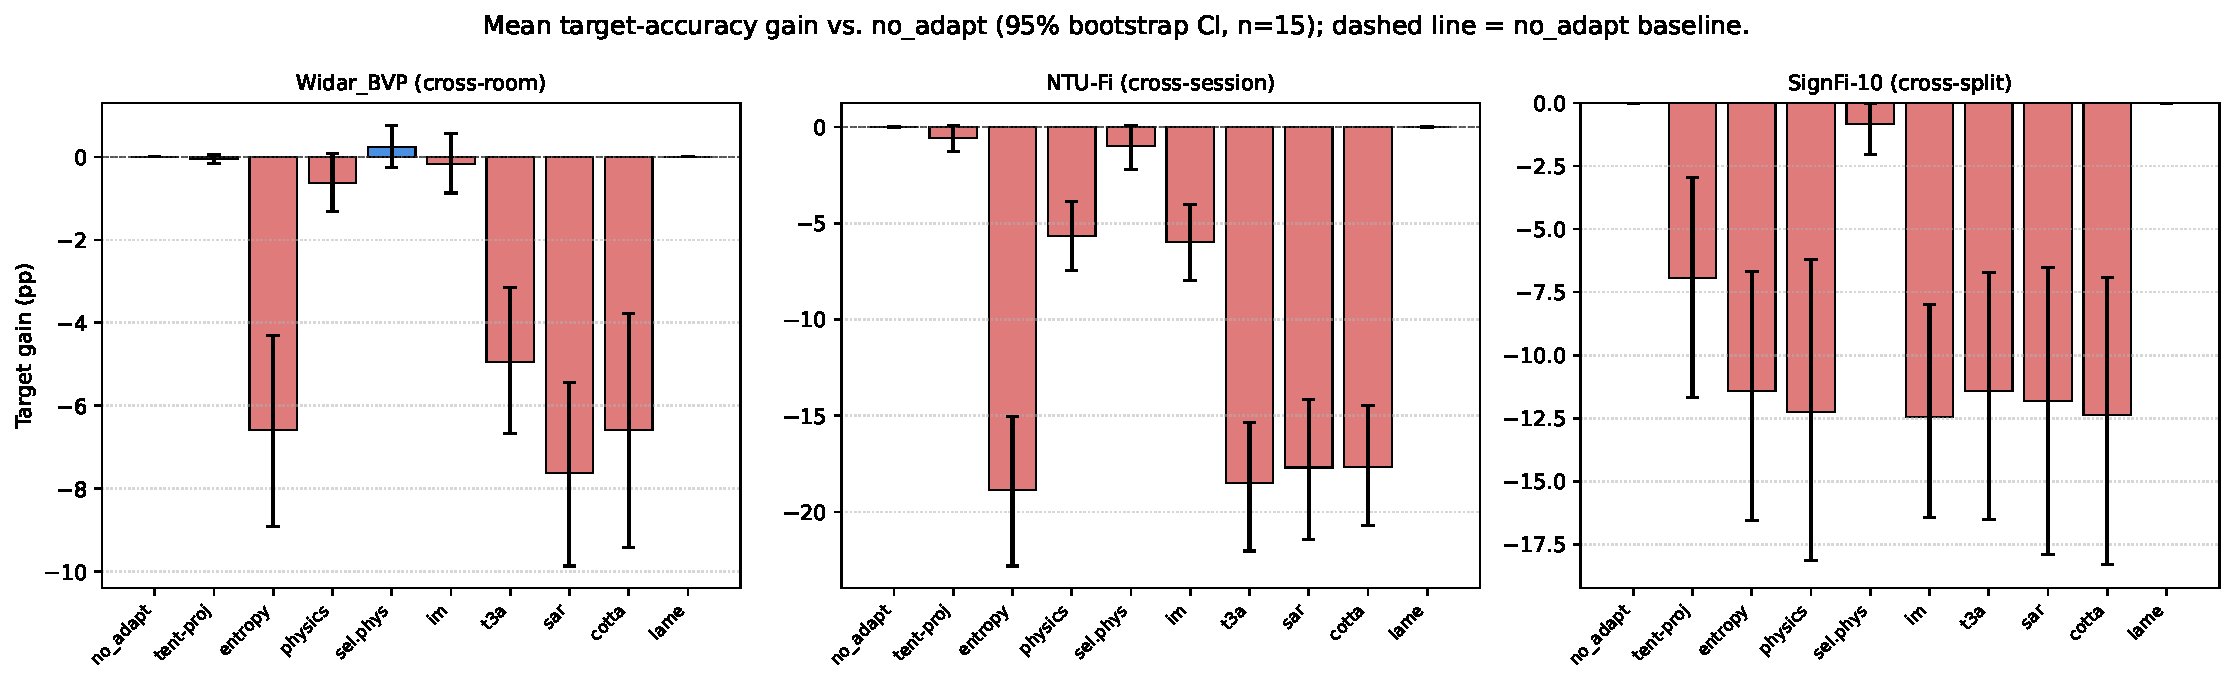
\includegraphics[width=\textwidth]{figures/fig1_method_comparison.pdf}
    \caption{Mean target-accuracy gain (pp, 95\% bootstrap CI) for all benchmark methods across Widar\_BVP, NTU-Fi, and SignFi-10 on the primary MLP backbone ($n{=}15$ per cell). Dashed line: \texttt{no\_adapt}. Bars below zero indicate negative adaptation. The \emph{faithful} BN-only TENT counterexample on MLP+BN (Table~\ref{tab:signfi_mlpbn}) is not in this figure because the primary-MLP port of TENT is \texttt{tent-proj}; the counterexample is examined separately in Section~\ref{sec:arch}.}
    \label{fig:comparison}
\end{figure}

\subsection{Source Calibration: Label Smoothing Ablation}

\begin{table}[h]
\centering
\caption{Label smoothing ablation on Widar\_BVP ($n{=}15$). Smoothing $\alpha{=}0.1$ reduces \texttt{physics\_tta} damage from $-$0.20 to $-$0.10~pp and lowers the negative adaptation rate from 0.60 to 0.47.}
\label{tab:smoothing}
\small
\begin{tabular}{lcccc}
\toprule
\textbf{Smoothing $\alpha$} & \textbf{Baseline} & \textbf{physics gain} & \textbf{tent gain} & \textbf{Neg Rate (phys)} \\
\midrule
0.0 (none) & 35.5\% & $-$0.20~pp & $+$0.01~pp & 0.60 \\
0.1 & 35.9\% & $-$0.10~pp & $+$0.00~pp & 0.47 \\
0.2 & 35.9\% & $-$0.36~pp & $-$0.04~pp & 0.60 \\
\bottomrule
\end{tabular}
\end{table}

At $\alpha{=}0.1$, \texttt{physics\_tta} damage is reduced ($-$0.20 $\to$ $-$0.10~pp) and negative adaptation rate drops from 0.60 to 0.47. The effect is modest and not statistically significant, but is directionally consistent with calibration literature~\cite{guo2017calibration,muller2019labelsmoothing}: reducing overconfidence limits the damage from entropy-based adaptation.

\subsection{Supervised Upper Bound and Synthetic-to-Real Gap}

A labelled-target oracle fine-tuned on Widar\_BVP (per held-out room, 5-fold CV, Adam lr=1e-3, 30 epochs of fine-tuning from the matched source checkpoint; 3 rooms $\times$ 3 seeds $= 9$ room/seed aggregates; \texttt{scripts/train\_supervised\_upper\_bound.py}; Appendix~\ref{app:upperbound}) improves mean target accuracy from $36.2\%$ (matched source-only) to $61.1\%$ under this protocol, a $+$24.9~pp supervised gap. The per-room gaps are strongly heterogeneous ($+$42.8 on room~2, $+$26.1 on room~0, $+$5.2 on room~1), which itself supports the shift-severity interpretation. The best unlabelled TTA gain on the primary MLP is $+$0.25~pp (\texttt{selective\_physics}), so unlabelled TTA in this protocol recovers $\approx$1\% of the supervised headroom. On controlled synthetic data with known physics parameters, \texttt{safe\_physics} achieves $+$8.0~pp ($d{=}+0.72$); the same physics-prior objective family yields $-$0.5~pp on real Widar (an $\approx$8.5~pp synthetic-to-real swing; Figure~\ref{fig:gap}).

\begin{figure}[t]
    \centering
    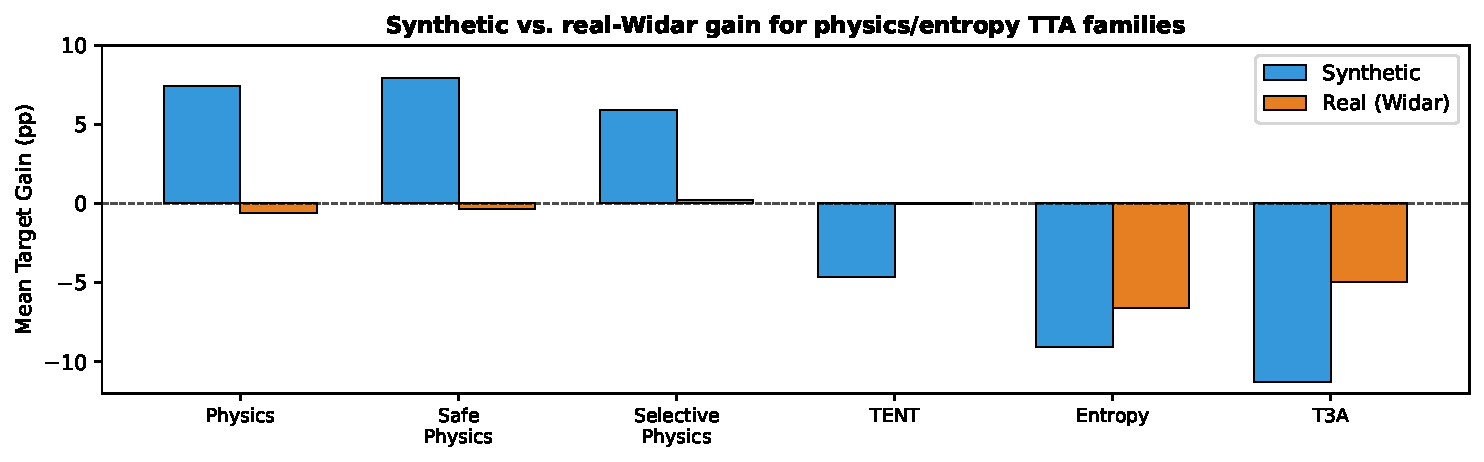
\includegraphics[width=0.85\textwidth]{figures/fig2_synthetic_real_gap.pdf}
    \caption{Synthetic vs.\ real gain for key methods. Physics-guided methods succeed with known parameters (blue) but fail on real data (orange).}
    \label{fig:gap}
\end{figure}

\subsection{Architecture: Faithful TENT Controls and SignFi Counterexample}
\label{sec:arch}

A key question is whether TTA's failure is due to the MLP's lack of BatchNorm. We implement \texttt{mlp\_bn} (MLP with BatchNorm in every layer) and run faithful TENT (BN-affine-only updates) alongside BN-reset. Table~\ref{tab:faithful_tent} summarises the three-way Widar comparison; Table~\ref{tab:signfi_mlpbn} gives the SignFi counterexample on the same MLP+BN backbone.

\begin{table}[h]
\centering
\caption{Architecture ablation on real Widar\_BVP. MLP and MLP+BN rows use $n{=}15$ paired observations (3 folds $\times$ 5 seeds); the CNN1D+BN row is an exploratory one-room probe with 3 seeds and is reported only as evidence that BN architectures do not automatically rescue TTA. MLP+BN raises the source-only baseline but no evaluated TTA method improves upon it within measurement noise; faithful BN-only TENT averages $-$0.61~pp on Widar.}
\label{tab:faithful_tent}
\small
\begin{tabular}{llcc}
\toprule
\textbf{Backbone} & \textbf{Method} & \textbf{Gain (pp)} & \textbf{Abs Acc} \\
\midrule
\multirow{3}{*}{MLP (no BN)} & \texttt{no\_adapt} & 0.00 & 35.7\% \\
 & \texttt{tent-proj} & $+$0.01 & 35.7\% \\
 & \texttt{physics} & $-$0.20 & 35.5\% \\
\midrule
\multirow{4}{*}{MLP+BN} & \texttt{no\_adapt} & 0.00 & \textbf{36.9\%} \\
 & \texttt{bn\_reset} & $-$1.11 & 35.8\% \\
 & \texttt{tent} (faithful, BN-only) & $-$0.61 & 36.4\% \\
 & \texttt{physics} & $-$0.55 & 36.4\% \\
\midrule
\multirow{2}{*}{CNN1D+BN (real, 1 room)} & \texttt{tent-proj} & $+$2.63 & --- \\
 & \texttt{physics} & $+$1.61 & --- \\
\bottomrule
\end{tabular}
\end{table}

\begin{table}[h]
\centering
\caption{MLP+BN on SignFi-10 ($n{=}15$): the same backbone that fails on Widar's hard cross-room shift succeeds dramatically on SignFi's milder shift.}
\label{tab:signfi_mlpbn}
\small
\begin{tabular}{lccc}
\toprule
\textbf{Method} & \textbf{Gain (pp)} & \textbf{95\% CI} & \textbf{Neg Rate} \\
\midrule
\texttt{tent} (faithful, BN-only) & \textbf{+21.1} & $[+13.1, +29.6]$ & \textbf{0.00} \\
\texttt{entropy} & $+$15.6 & $[+8.2, +22.8]$ & 0.07 \\
\texttt{physics} & $+$12.3 & $[+4.8, +20.2]$ & 0.13 \\
\bottomrule
\end{tabular}
\end{table}

\textbf{Key finding.} The \emph{same} BN-equipped backbone fails on Widar ($-$0.61~pp) and succeeds on SignFi ($+$21.1~pp). BN availability alone does not explain the hard-shift failure: TTA outcomes depend on the interaction between shift severity (Widar 52~pp domain gap vs.\ SignFi 14~pp), source calibration, and architecture. Per-row MLP vs MLP+BN means/stds (the full \texttt{arch\_3way} table) and the one-room CNN1D+BN probe are reported in Appendix~\ref{app:cnn1d_probe}/\ref{app:arch_full}.
